% This file was created with tikzplotlib v0.10.1.
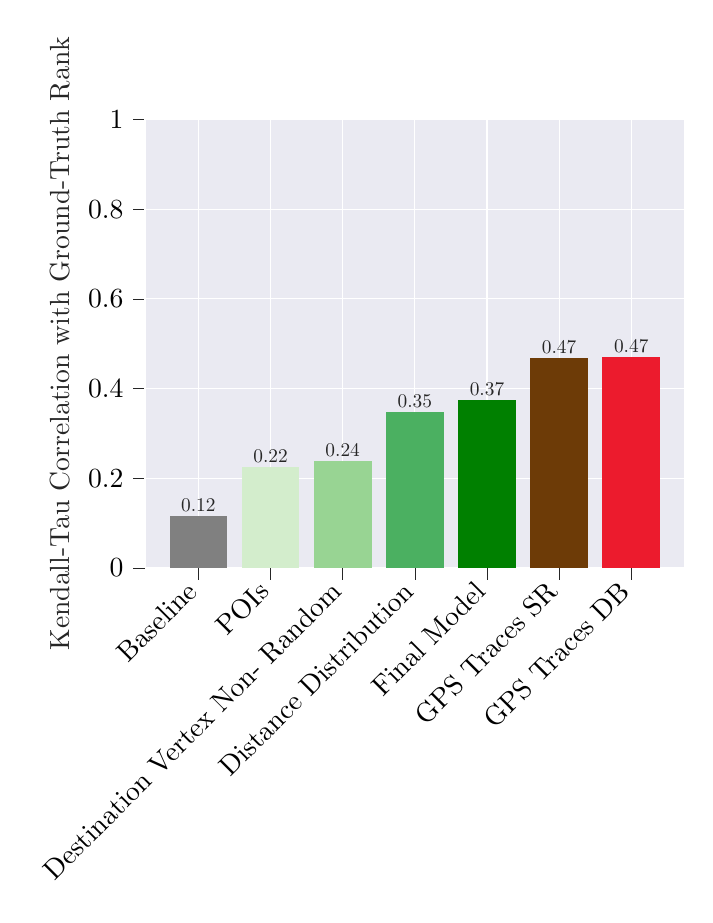
\begin{tikzpicture}

\definecolor{crimson2362745}{RGB}{236,27,45}
\definecolor{darkseagreen152212147}{RGB}{152,212,147}
\definecolor{darkslategrey38}{RGB}{38,38,38}
\definecolor{gainsboro211237204}{RGB}{211,237,204}
\definecolor{green}{RGB}{0,128,0}
\definecolor{grey}{RGB}{128,128,128}
\definecolor{lavender234234242}{RGB}{234,234,242}
\definecolor{mediumseagreen7517697}{RGB}{75,176,97}
\definecolor{saddlebrown109597}{RGB}{109,59,7}

\begin{axis}[
axis background/.style={fill=lavender234234242},
axis line style={white},
tick align=outside,
tick pos=left,
x grid style={white},
xmajorgrids,
xmin=-0.74, xmax=6.74,
xtick style={color=darkslategrey38},
xtick={0,1,2,3,4,5,6},
xticklabel style={rotate=45.0,anchor=east},
xticklabels={
  Baseline,
  POIs,
  Destination
Vertex Non-
Random,
  Distance
Distribution,
  Final Model,
  GPS Traces SR,
  GPS Traces DB
},
y grid style={white},
ylabel=\textcolor{darkslategrey38}{Kendall-Tau Correlation with Ground-Truth Rank},
ymajorgrids,
ymin=0, ymax=1,
ytick style={color=darkslategrey38}
]
\draw[draw=none,fill=grey,line width=0.12pt] (axis cs:-0.4,0) rectangle (axis cs:0.4,0.115942028985507);
\draw[draw=none,fill=gainsboro211237204,line width=0.12pt] (axis cs:0.6,0) rectangle (axis cs:1.4,0.22463768115942);
\draw[draw=none,fill=darkseagreen152212147,line width=0.12pt] (axis cs:1.6,0) rectangle (axis cs:2.4,0.239130434782609);
\draw[draw=none,fill=mediumseagreen7517697,line width=0.12pt] (axis cs:2.6,0) rectangle (axis cs:3.4,0.347826086956522);
\draw[draw=none,fill=green,line width=0.12pt] (axis cs:3.6,0) rectangle (axis cs:4.4,0.373866314449923);
\draw[draw=none,fill=saddlebrown109597,line width=0.12pt] (axis cs:4.6,0) rectangle (axis cs:5.4,0.468240335573205);
\draw[draw=none,fill=crimson2362745,line width=0.12pt] (axis cs:5.6,0) rectangle (axis cs:6.4,0.471014492753623);
\draw (axis cs:0,0.125942028985507) node[
  scale=0.7,
  anchor=base,
  text=darkslategrey38,
  rotate=0.0
]{0.12};
\draw (axis cs:1,0.23463768115942) node[
  scale=0.7,
  anchor=base,
  text=darkslategrey38,
  rotate=0.0
]{0.22};
\draw (axis cs:2,0.249130434782609) node[
  scale=0.7,
  anchor=base,
  text=darkslategrey38,
  rotate=0.0
]{0.24};
\draw (axis cs:3,0.357826086956522) node[
  scale=0.7,
  anchor=base,
  text=darkslategrey38,
  rotate=0.0
]{0.35};
\draw (axis cs:4,0.383866314449923) node[
  scale=0.7,
  anchor=base,
  text=darkslategrey38,
  rotate=0.0
]{0.37};
\draw (axis cs:5,0.478240335573205) node[
  scale=0.7,
  anchor=base,
  text=darkslategrey38,
  rotate=0.0
]{0.47};
\draw (axis cs:6,0.481014492753623) node[
  scale=0.7,
  anchor=base,
  text=darkslategrey38,
  rotate=0.0
]{0.47};
\end{axis}

\end{tikzpicture}
